% XCircuit output "bloques.tex" for LaTeX input from bloques.ps
\def\putbox#1#2#3#4{\makebox[0in][l]{\makebox[#1][l]{}\raisebox{\baselineskip}[0in][0in]{\raisebox{#2}[0in][0in]{\scalebox{#3}{#4}}}}}
\def\rightbox#1{\makebox[0in][r]{#1}}
\def\centbox#1{\makebox[0in]{#1}}
\def\topbox#1{\raisebox{-0.60\baselineskip}[0in][0in]{#1}}
\def\midbox#1{\raisebox{-0.20\baselineskip}[0in][0in]{#1}}
   \scalebox{1}{
   \normalsize
   \parbox{7.30729in}{
   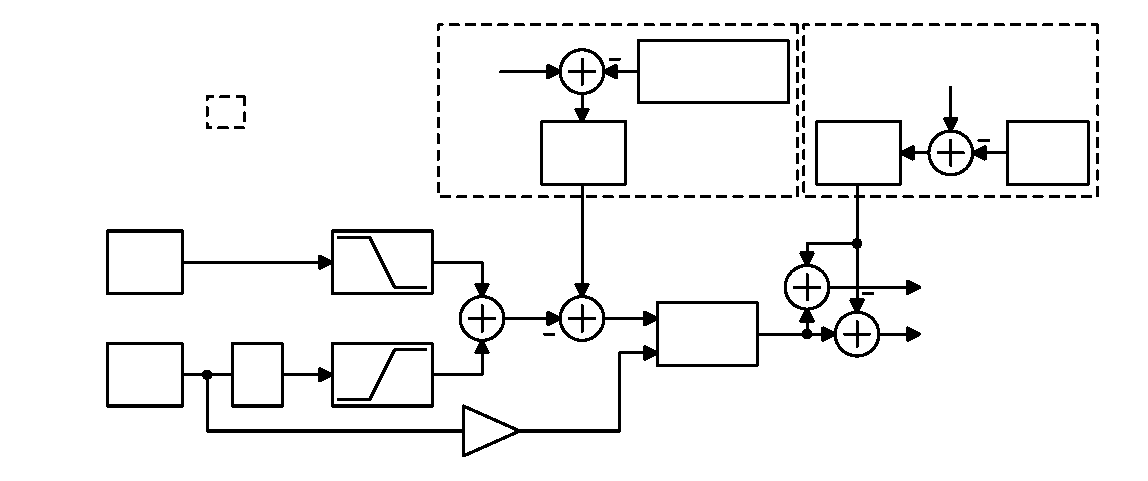
\includegraphics[scale=1]{bloques}\\
   % translate x=649 y=336 scale 0.38
   \putbox{1.60in}{0.43in}{1.20}{\centbox{\midbox{$\int$}}}%
   \putbox{2.44in}{1.43in}{1.20}{\centbox{LPF}}%
   \putbox{2.44in}{0.68in}{1.20}{\centbox{HPF}}%
   \putbox{0.85in}{1.26in}{1.20}{\centbox{\midbox{$\theta_m$}}}%
   \putbox{0.85in}{1.10in}{1.20}{\centbox{\midbox{Accel}}}%
   \putbox{0.85in}{0.35in}{1.20}{\centbox{\midbox{Gyro}}}%
   \putbox{0.85in}{0.51in}{1.20}{\centbox{\midbox{$\dot{\theta}_m$}}}%
   \putbox{3.44in}{0.95in}{1.20}{\centbox{\midbox{$\theta_e$}}}%
   \putbox{4.60in}{0.70in}{1.20}{\centbox{\midbox{PID}}}%
   \putbox{3.79in}{1.39in}{1.20}{\midbox{$\theta_{ref}$}}%
   \putbox{5.62in}{1.47in}{1.20}{\midbox{offset}}%
   \putbox{6.04in}{1.01in}{1.20}{\midbox{PWMA}}%
   \putbox{6.04in}{0.70in}{1.20}{\midbox{PWMB}}%
   \putbox{4.64in}{2.54in}{1.20}{\centbox{\midbox{Encoders}}}%
   \putbox{4.64in}{2.35in}{1.20}{\centbox{\midbox{(velocidad)}}}%
   \putbox{3.77in}{1.91in}{1.20}{\centbox{\midbox{PI}}}%
   \putbox{3.21in}{2.47in}{1.20}{\rightbox{\midbox{$v_{ref}$}}}%
   \putbox{5.60in}{1.91in}{1.20}{\centbox{\midbox{PI}}}%
   \putbox{6.85in}{1.99in}{1.20}{\centbox{\midbox{Gyro}}}%
   \putbox{6.83in}{1.81in}{1.20}{\centbox{\midbox{$\dot{\psi}$}}}%
   \putbox{6.25in}{2.47in}{1.20}{\centbox{\midbox{$\dot{\psi}_{ref}$}}}%
   \putbox{0.96in}{2.12in}{1.20}{\centbox{Ideas}}%
   } % close 'parbox'
   } % close 'scalebox'
   \vspace{-\baselineskip} % this is not necessary, but looks better
